\documentclass{beamer}
\usepackage[utf8]{inputenc}

\usetheme{Madrid}
\usecolortheme{default}
\usepackage{amsmath,amssymb,amsfonts,amsthm}
\usepackage{txfonts}
\usepackage{tkz-euclide}
\usepackage{listings}
\usepackage{adjustbox}
\usepackage{array}
\usepackage{tabularx}
\usepackage{gvv}
\usepackage{lmodern}
\usepackage{circuitikz}
\usepackage{tikz}
\usepackage{graphicx}
\usepackage{gensymb} % For using \degree symbol
\usepackage{enumitem}

\setbeamertemplate{page number in head/foot}[totalframenumber]

% Title Information
\title{5.2.6}
\date{October 10, 2025}
\author{ADHARVAN KSHATHRIYA BOMMAGANI - EE25BTECH11003}

\begin{document}

% Title Slide
\frame{\titlepage}

% Question Slide
\begin{frame}{Question}
Solve the following system of linear equations using Gaussian elimination and matrices:
\begin{center}
    2x - 3y = 8 \\
    4x - 6y = 9
\end{center}
\end{frame}

% Solution Step 1: Augmented Matrix
\begin{frame}{Theoretical Solution}
First, we represent the system of equations as an augmented matrix.
\begin{align}
\myaugvec{2}{
2 & -3 & 8 \\
4 & -6 & 9
}
\end{align}
\bigskip
Next, we apply the row operation $R_2 \to R_2 - 2R_1$ to create a zero in the first column of the second row:
\begin{align}
\myaugvec{2}{
2 & -3 & 8 \\
0 & 0 & -7
}
\end{align}

\end{frame}

% Solution Step 2: Interpretation and Conclusion
\begin{frame}{Theoretical Solution}
Now, we translate the second row of the resulting matrix back into an equation:
\begin{align}
    0x + 0y = -7
\end{align}
This simplifies to the statement:
\begin{align}
    0 = -7
\end{align}
This statement is a contradiction, as 0 is not equal to -7.
\bigskip

Because the process leads to a contradiction, the original system of equations is described as \textbf{inconsistent}. This means there is no pair of values for $x$ and $y$ that can satisfy both equations simultaneously.
\bigskip
Therefore, the system has \textbf{no solution}.
\end{frame}

% Plot Slide
\begin{frame}{Plot}
\begin{figure}[H]
    \centering
    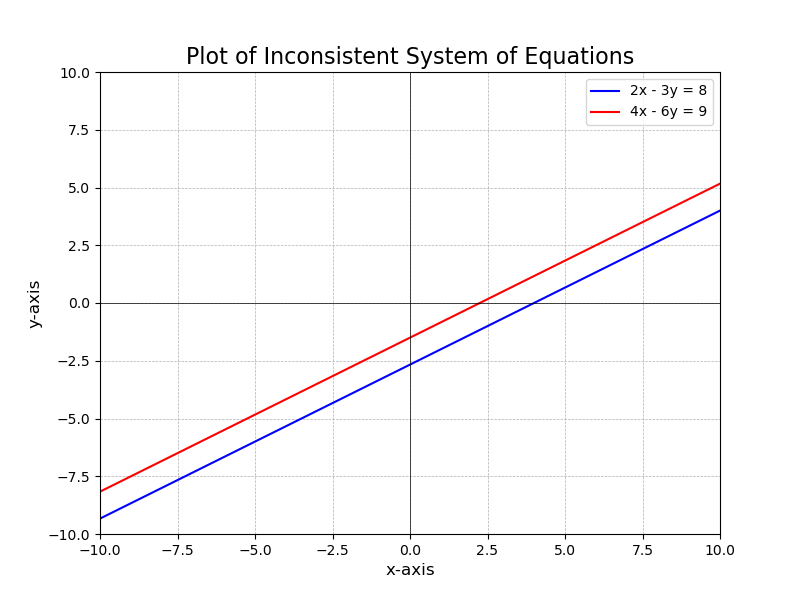
\includegraphics[width=0.7\columnwidth]{figs/fig1.png}
    \caption{figure for 5.2.6}
    \label{fig:lines}
\end{figure}
\end{frame}

\end{document}